\documentclass[17pt,compress]{beamer}
\usepackage{beamerthemesplit}
\mode<presentation>
{
  \usetheme{Warsaw}
  \setbeamercovered{transparent}
  \setbeamertemplate{navigation symbols}{}
}
% Taken from Fernando's slides.
\usepackage{ae,aecompl}
\usepackage[scaled=.95]{helvet}

\usepackage[english]{babel}
\usepackage[latin1]{inputenc}
\usepackage[T1]{fontenc}

\newcounter{saveenumi}
\newcommand{\seti}{\setcounter{saveenumi}{\value{enumi}}}
\newcommand{\conti}{\setcounter{enumi}{\value{saveenumi}}}


\definecolor{blue}{rgb}{0.16,0.32,0.75}
\setbeamercolor{structure}{fg=blue}
\author[FOSSEE]{}
\institute[IIT Bombay]{}
\date[]{}
% \setbeamercovered{transparent}

% theme split
\usepackage{verbatim}
\newenvironment{colorverbatim}[1][]%
{%
\color{blue}
\verbatim
}%
{%
\endverbatim
}%

\usepackage{mathpazo,courier,euler}
\usepackage{listings}
\lstset{language=sh,
    basicstyle=\ttfamily\bfseries,
  showstringspaces=false,
  keywordstyle=\color{black}\bfseries}

% logo
\logo{
\includegraphics[height=1.30 cm]{3t-logo.pdf}}
\logo{
\includegraphics[height=1.30 cm]{fossee-logo.png}

\hspace{7.5cm}

\includegraphics[scale=0.3]{fossee-logo.png}\\
\hspace{281pt}

\includegraphics[scale=0.80]{3t-logo.pdf}}

\begin{document}

\sffamily \bfseries
\title
[Other types of Plots]
{Python - Other types of Plots}
\author
[FOSSEE, IIT - Bombay]
{\small Talk to a Teacher\\{\color{blue}\url{http://spoken-tutorial.org}}\\National Mission on Education
 through ICT\\{\color{blue}\url{http://sakshat.ac.in}} \\[0.5cm]{\tiny Script by: Hardik ghaghada \\ Naration by: Hardik Ghaghada \\ 13 August 2015}}

% slide 1
\begin{frame}
   \titlepage
\end{frame}
%%%%%%%%%%%%%%%%%%%%%%%%%%%%%%%%%%%%%%%%%%%%%%%%%%%%%%%%%%%%%%%%%%%%%%%%%%%%%%%%
\begin{frame}
\frametitle{Objectives}
\label{sec-2}

  In this tutorial, we will learn -\pause

\begin{itemize}
\item Creating scatter plot\pause
\item Creating pie charts\pause
\item Creating bar charts\pause
\item Creating log-log plots\pause
\item Use the \texttt{matplotlib} help
\end{itemize}
\end{frame}
%%%%%%%%%%%%%%%%%%%%%%%%%%%%%%%%%%%%%%%%%%%%%%%%%%%%%%%%%%%%%%%%%%%%%%%%%%%%%%%%
\begin{frame}
\frametitle{System Specifications}\pause
\begin{itemize}
\item Slackware Linux 14.1\pause
\item \texttt{Python 2.7.5} \pause
\item \texttt{IPython 2.3.0}
\end{itemize}
\end{frame}
%%%%%%%%%%%%%%%%%%%%%%%%%%%%%%%%%%%%%%%%%%%%%%%%%%%%%%%%%%%%%%%%%%%%%%%%%%%%%%%%
\begin{frame}
\frametitle{Pre-requisites}
\label{sec-3}
Spoken tuorial on -
\begin{itemize}
\item Loading Data from Files.\pause
\item Plotting Data.
\end{itemize}
\end{frame}
%%%%%%%%%%%%%%%%%%%%%%%%%%%%%%%%%%%%%%%%%%%%%%%%%%%%%%%%%%%%%%%%%%%%%%%%%%%%%%%%
\begin{frame}
\frametitle{Exercise 1: Scatter plot}
\label{sec-5}
Plot a scatter plot showing the percentage profit of Company A from the year 2000
to 2010. The data for the same is available in the file `company-a-data.txt'.
\end{frame}
\begin{frame}[fragile]
\frametitle{scatter() function}
\label{sec-6}
\begin{itemize}
\item Syntax: \texttt{scatter(x,y)}\pause
\begin{itemize}
\item x, a sequence of data\pause
\item y, a sequence of data, the same length of x\pause
\end{itemize}
\end{itemize}
Example: \texttt{scatter(year, profit)}
\end{frame}
%%%%%%%%%%%%%%%%%%%%%%%%%%%%%%%%%%%%%%%%%%%%%%%%%%%%%%%%%%%%%%%%%%%%%%%%%%%%%%%%
\begin{frame}[fragile]
\frametitle{Exercise 2: Scatter plot}
\label{sec-7}
\begin{itemize}
\item Plot a scatter plot of the same data in `company-a-data.txt' with red diamond markers.\pause
\item Clue - try \texttt{scatter?} in your \texttt{ipython} interpreter
\end{itemize}
%%%%%%%%%%%%%%%%%%%%%%%%%%%%%%%%%%%%%%%%%%%%%%%%%%%%%%%%%%%%%%%%%%%%%%%%%%%%%%%%
\end{frame}
\begin{frame}
\frametitle{Pie chart}
\label{sec-8}
Pie chart - a circle graph divided into sectors, illustrating proportion.
\end{frame}
%%%%%%%%%%%%%%%%%%%%%%%%%%%%%%%%%%%%%%%%%%%%%%%%%%%%%%%%%%%%%%%%%%%%%%%%%%%%%%%%
\begin{frame}[fragile]
\frametitle{Exercise 3: Pie chart}
\label{sec-9}
Plot a pie chart representing the profit percentage of company A, with the data
from the file `company-a-data.txt'.\pause
\begin{verbatim}
\end{verbatim}
\emph{(we can reuse the data in lists year and profit)}
\end{frame}
%%%%%%%%%%%%%%%%%%%%%%%%%%%%%%%%%%%%%%%%%%%%%%%%%%%%%%%%%%%%%%%%%%%%%%%%%%%%%%%%
\begin{frame}[fragile]
\frametitle{pie() function}
\label{sec-10}
\begin{itemize}
\item Syntax: \texttt{pie(values,labels=labels)}\pause
\begin{itemize}
\item values, the data to be plotted\pause
\item labels, the label for each wedge in the pie chart\pause
\end{itemize}

\item Example: \texttt{pie(profit,labels=year)}
\end{itemize}
\end{frame}
%%%%%%%%%%%%%%%%%%%%%%%%%%%%%%%%%%%%%%%%%%%%%%%%%%%%%%%%%%%%%%%%%%%%%%%%%%%%%%%%
\begin{frame}[fragile]
\frametitle{Exercise 4: Pie chart}
\label{sec-11}
\begin{itemize}
\item Plot a pie chart with the same data with colors for each wedges as white, red,
magenta, yellow, blue, green, cyan, yellow, magenta, and blue.\pause
\item \textbf{Clue} - try \texttt{pie?} in your \texttt{ipython} interpreter
\end{itemize}
\end{frame}
%%%%%%%%%%%%%%%%%%%%%%%%%%%%%%%%%%%%%%%%%%%%%%%%%%%%%%%%%%%%%%%%%%%%%%%%%%%%%%%%
\begin{frame}
\frametitle{Bar chart}
\label{sec-12}
Bar chart - a chart with rectangular bars with lengths proportional
to the values that they represent.
\end{frame}
%%%%%%%%%%%%%%%%%%%%%%%%%%%%%%%%%%%%%%%%%%%%%%%%%%%%%%%%%%%%%%%%%%%%%%%%%%%%%%%%
\begin{frame}[fragile]
\frametitle{Exercise 5: Bar chart}
\label{sec-13}
Plot a bar chart representing the profit percentage of company A, with the data
from the file `company-a-data.txt'.
\begin{verbatim}
\end{verbatim}
\emph{(we can reuse the data in lists year and profit)}
\end{frame}
%%%%%%%%%%%%%%%%%%%%%%%%%%%%%%%%%%%%%%%%%%%%%%%%%%%%%%%%%%%%%%%%%%%%%%%%%%%%%%%%
\begin{frame}[fragile]
\frametitle{bar() function}
\label{sec-14}
\begin{itemize}
\item Syntax: \texttt{bar(x, y)}\pause
\begin{itemize}
\item x, a sequence of data\pause
\item y, a sequence of data, the same length of x\pause
\end{itemize}
\item Example: \texttt{bar(year, profit)}
\end{itemize}
\end{frame}
%%%%%%%%%%%%%%%%%%%%%%%%%%%%%%%%%%%%%%%%%%%%%%%%%%%%%%%%%%%%%%%%%%%%%%%%%%%%%%%%
\begin{frame}
\frametitle{Exercise 6: Bar chart}
\label{sec-15}
\begin{itemize}
\item Plot a bar chart which is not filled and which is hatched with
45$^o$ slanting lines as shown in the image.
\item The data for the chart may be obtained from the file `company-a-data.txt.'
\end{itemize}
\end{frame}
%%%%%%%%%%%%%%%%%%%%%%%%%%%%%%%%%%%%%%%%%%%%%%%%%%%%%%%%%%%%%%%%%%%%%%%%%%%%%%%%
\begin{frame}
\frametitle{Exercise 6: Bar chart}
\label{sec-15}
\begin{center}
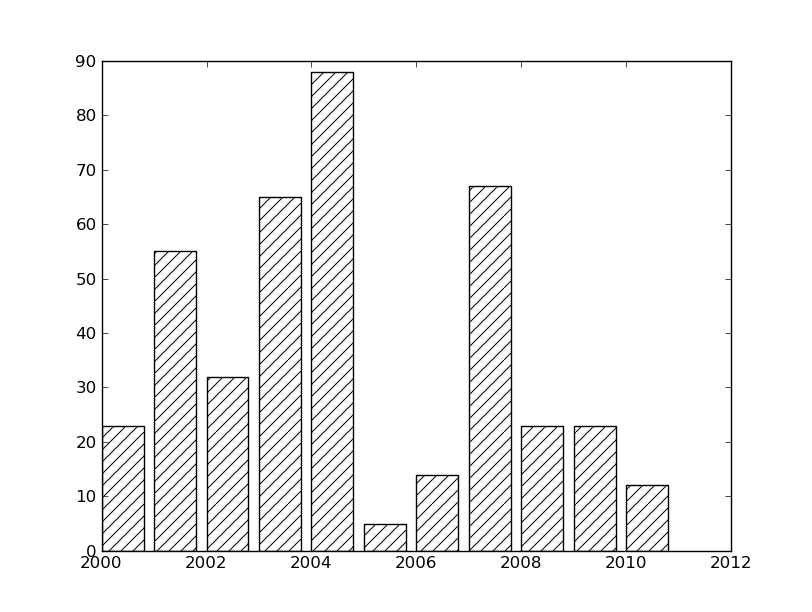
\includegraphics[scale=0.3]{bar-chart-hatch.png}
\end{center}
\begin{itemize}
\item {Clue} - try \texttt{bar?} in your \texttt{ipython} interpreter
\end{itemize}
\end{frame}
%%%%%%%%%%%%%%%%%%%%%%%%%%%%%%%%%%%%%%%%%%%%%%%%%%%%%%%%%%%%%%%%%%%%%%%%%%%%%%%%
\begin{frame}
\frametitle{Log-log graph}
\label{sec-16}
\begin{itemize}
\item Log-log graph
\begin{itemize}
\item 2-dimensional graph.\pause
\item uses logarithmic scales on both axes.\pause
\item graph appears as straight line due to non-linear scaling.
\end{itemize}
\end{itemize}
\end{frame}
%%%%%%%%%%%%%%%%%%%%%%%%%%%%%%%%%%%%%%%%%%%%%%%%%%%%%%%%%%%%%%%%%%%%%%%%%%%%%%%%
\begin{frame}
\frametitle{Exercise 7:}
\label{sec-17}
Plot a log-log chart of $y = 5x^3$ for $x$ from 1-20.
\end{frame}
%%%%%%%%%%%%%%%%%%%%%%%%%%%%%%%%%%%%%%%%%%%%%%%%%%%%%%%%%%%%%%%%%%%%%%%%%%%%%%%%
\begin{frame}[fragile]
\frametitle{loglog()function}
\label{sec-18}
\begin{itemize}
\item Syntax: \texttt{loglog(x, y)}\pause
\begin{itemize}
\item \texttt{x}, a sequence of data\pause
\item \texttt{y}, a sequence of data, the same length of \texttt{x}
\end{itemize}
\end{itemize}
\end{frame}
%%%%%%%%%%%%%%%%%%%%%%%%%%%%%%%%%%%%%%%%%%%%%%%%%%%%%%%%%%%%%%%%%%%%%%%%%%%%%%%%
\begin{frame}
\frametitle{Getting help on matplotlib}
\label{sec-19}
\begin{itemize}
\item Help
	\begin{itemize}
	\item \url{matplotlib.sourceforge.net/contents.html}\pause
	\end{itemize}
\item More plots
	\begin{itemize}
	\item \url{matplotlib.sourceforge.net/users/screenshots.html}\pause
	\item \url{matplotlib.sourceforge.net/gallery.html}
	\end{itemize}
\end{itemize}
\end{frame}
%%%%%%%%%%%%%%%%%%%%%%%%%%%%%%%%%%%%%%%%%%%%%%%%%%%%%%%%%%%%%%%%%%%%%%%%%%%%%%%%
\begin{frame}
\frametitle{Summary}
\label{sec-20}
In this tutorial, we learnt to -
\begin{itemize}
\item Plot a scatter plot using \texttt{scatter()} function
\item Plot a pie chart using \texttt{pie()} function
\end{itemize}
\end{frame}
%%%%%%%%%%%%%%%%%%%%%%%%%%%%%%%%%%%%%%%%%%%%%%%%%%%%%%%%%%%%%%%%%%%%%%%%%%%%%%%%
\begin{frame}
\frametitle{Summary contd..}
\label{sec-20}
\begin{itemize}
\item Plot a bar chart using \texttt{bar()} function
\item Plot a log-log graph using \texttt{loglog()} function
\item Access the \texttt{matplotlib} online help.
\end{itemize}
\end{frame}
%%%%%%%%%%%%%%%%%%%%%%%%%%%%%%%%%%%%%%%%%%%%%%%%%%%%%%%%%%%%%%%%%%%%%%%%%%%%%%%%
\begin{frame}
\frametitle{Evaluation}
\label{sec-21.1}
\begin{enumerate}
\item \texttt{scatter(x, y, color='blue', marker='d')} \pause
and \\
\texttt{plot(x, y,color='b', marker='d')}\pause \\ Does exactly the same? (True or False)
\seti
\end{enumerate}
\end{frame}
%%%%%%%%%%%%%%%%%%%%%%%%%%%%%%%%%%%%%%%%%%%%%%%%%%%%%%%%%%%%%%%%%%%%%%%%%%%%%%%%
\begin{frame}
\frametitle{Evaluation contd..}
\label{sec-21.2}
\begin{enumerate}
\conti
\item What statement can be issued to generate a bar chart with vertical
line hatching.\pause
\begin{itemize}
\item bar(x, y, color = 'w', hatch = '/')
\item bar(x, y, fill = False, hatch = '//')
\item bar(x, y, fill = False, hatch = '|')
\item bar(x, y, color = 'w', hatch = '$\backslash$')
\end{itemize}
\end{enumerate}
\end{frame}
%%%%%%%%%%%%%%%%%%%%%%%%%%%%%%%%%%%%%%%%%%%%%%%%%%%%%%%%%%%%%%%%%%%%%%%%%%%%%%%%
\begin{frame}
\frametitle{Solutions}
\label{sec-22}
\begin{enumerate}
\item False\pause
\item bar(x, y, fill = False, hatch = '|')
\end{enumerate}
\end{frame}
%%%%%%%%%%%%%%%%%%%%%%%%%%%%%%%%%%%%%%%%%%%%%%%%%%%%%%%%%%%%%%%%%%%%%%%%%%%%%%%%
\begin{frame}
\frametitle{FOSSEE}
{\color{blue}Free and Open-source Software for \\Science and Engineering Education} \\
\begin{itemize}
\item Goal - enabling all to use open source software tools
\item For more details, please visit {\color{blue}\url{http://fossee.in/}}
\end{itemize}
\end{frame}
%%%%%%%%%%%%%%%%%%%%%%%%%%%%%%%%%%%%%%%%%%%%%%%%%%%%%%%%%%%%%%%%%%%%%%%%%%%%%%%%
\begin{frame}
\frametitle{About the Spoken Tutorial Project}
\begin{itemize}
\item Watch the video available at {\color{blue}http://spoken-tutorial.org /What\_is\_a\_Spoken\_Tutorial}
\item It summarises the Spoken Tutorial project \pause
\item If you do not have good bandwidth, you can download and watch it
\end{itemize}
\end{frame}
%%%%%%%%%%%%%%%%%%%%%%%%%%%%%%%%%%%%%%%%%%%%%%%%%%%%%%%%%%%%%%%%%%%%%%%%%%%%%%%%
\begin{frame}
\frametitle{Spoken Tutorial Workshops}The Spoken Tutorial Project Team 
\begin{itemize}
\item Conducts workshops using spoken tutorials 
\item Gives certificates to those who pass an online test 
\item For more details, please write to \\ \hspace {0.5cm}{\color{blue}contact@spoken-tutorial.org}
\end{itemize}
\end{frame}
%%%%%%%%%%%%%%%%%%%%%%%%%%%%%%%%%%%%%%%%%%%%%%%%%%%%%%%%%%%%%%%%%%%%%%%%%%%%%%%%
\begin{frame}
\frametitle{Acknowledgements}
\begin{itemize}
\item Spoken Tutorial Project is a part of the Talk to a Teacher  project 
\item It is supported by the National Mission on Education through  ICT, MHRD, Government of India 
\item More information on this Mission is available at: \\{\color{blue}http://spoken-tutorial.org /NMEICT-Intro}
\end{itemize}
\end{frame}
%%%%%%%%%%%%%%%%%%%%%%%%%%%%%%%%%%%%%%%%%%%%%%%%%%%%%%%%%%%%%%%%%%%%%%%%%%%%%%%%
\begin{frame}

  \begin{block}{}
  \begin{center}
  \textcolor{blue}{\Large THANK YOU!} 
  \end{center}
  \end{block}
\begin{block}{}
  \begin{center}
    For more Information, visit our website\\
    \url{http://fossee.in/}
  \end{center}  
  \end{block}
\end{frame}
%%%%%%%%%%%%%%%%%%%%%%%%%%%%%%%%%%%%%%%%%%%%%%%%%%%%%%%%%%%%%%%%%%%%%%%%%%%%%%%%
\end{document}
